% Figure 3: Architecture Comparison - CPU vs NPU
\documentclass[tikz,border=10pt]{standalone}
\usepackage{tikz}
\usetikzlibrary{shapes,arrows,positioning,calc,fit,backgrounds,matrix}

\begin{document}
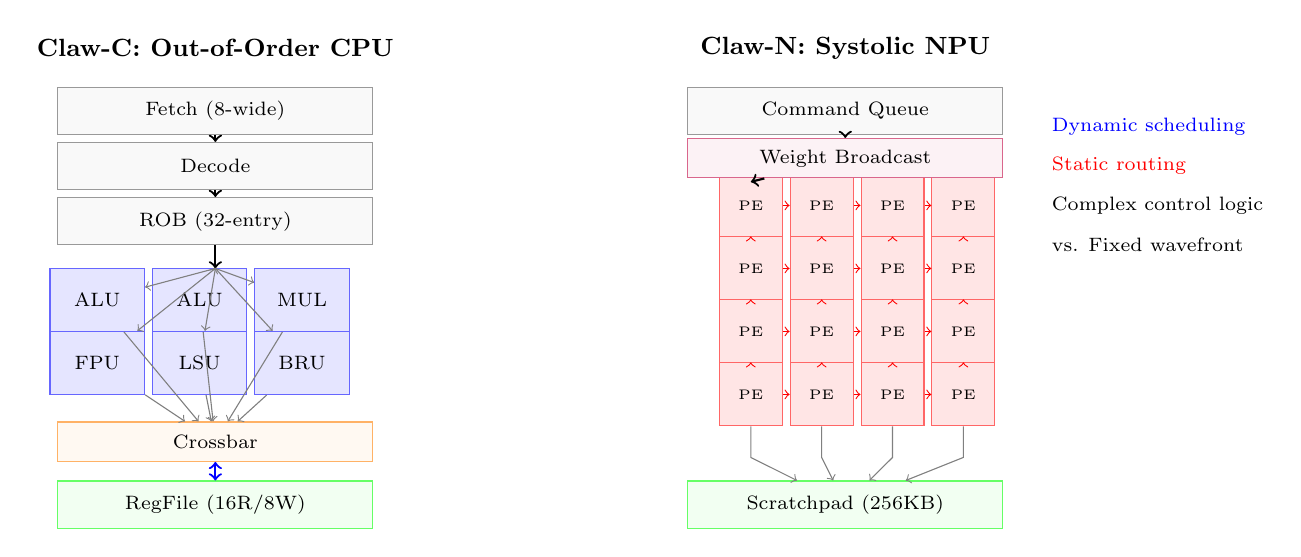
\begin{tikzpicture}[
    node distance=0.8cm,
    cpueu/.style={rectangle, draw=blue!60, fill=blue!10, minimum width=1.2cm,
                  minimum height=0.8cm, text centered, font=\scriptsize},
    npueu/.style={rectangle, draw=red!60, fill=red!10, minimum width=0.8cm,
                  minimum height=0.8cm, text centered, font=\tiny},
    label/.style={font=\bfseries\small}
]

% CPU Architecture (Left)
\node[label] at (-4, 4) {Claw-C: Out-of-Order CPU};

% Frontend
\node[rectangle, draw=black!40, fill=gray!5, minimum width=4cm, minimum height=0.6cm] (fetch) at (-4, 3.2) {\scriptsize Fetch (8-wide)};
\node[rectangle, draw=black!40, fill=gray!5, minimum width=4cm, minimum height=0.6cm] (decode) at (-4, 2.5) {\scriptsize Decode};
\node[rectangle, draw=black!40, fill=gray!5, minimum width=4cm, minimum height=0.6cm] (rob) at (-4, 1.8) {\scriptsize ROB (32-entry)};

% EU Pool
\node[cpueu] (alu0) at (-5.5, 0.8) {ALU};
\node[cpueu] (alu1) at (-4.2, 0.8) {ALU};
\node[cpueu] (mul0) at (-2.9, 0.8) {MUL};
\node[cpueu] (fpu0) at (-5.5, 0) {FPU};
\node[cpueu] (lsu0) at (-4.2, 0) {LSU};
\node[cpueu] (bru0) at (-2.9, 0) {BRU};

% Crossbar
\node[rectangle, draw=orange!60, fill=orange!5, minimum width=4cm, minimum height=0.5cm] (xbar_cpu) at (-4, -1) {\scriptsize Crossbar};

% RegFile
\node[rectangle, draw=green!60, fill=green!5, minimum width=4cm, minimum height=0.6cm] (rf_cpu) at (-4, -1.8) {\scriptsize RegFile (16R/8W)};

% Arrows
\draw[->, thick] (fetch) -- (decode);
\draw[->, thick] (decode) -- (rob);
\draw[->, thick] (rob) -- (-4, 1.2);
\draw[->, gray] (-4, 1.2) -- (alu0);
\draw[->, gray] (-4, 1.2) -- (alu1);
\draw[->, gray] (-4, 1.2) -- (mul0);
\draw[->, gray] (-4, 1.2) -- (fpu0);
\draw[->, gray] (-4, 1.2) -- (lsu0);
\draw[->, gray] (-4, 1.2) -- (bru0);

\foreach \eu in {alu0, alu1, mul0, fpu0, lsu0, bru0} {
    \draw[->, gray] (\eu) -- (xbar_cpu);
}

\draw[<->, thick, blue] (xbar_cpu) -- (rf_cpu);

% NPU Architecture (Right)
\node[label] at (4, 4) {Claw-N: Systolic NPU};

% Command Queue
\node[rectangle, draw=black!40, fill=gray!5, minimum width=4cm, minimum height=0.6cm] (cmdq) at (4, 3.2) {\scriptsize Command Queue};

% Systolic Array (4x4 for visualization)
\foreach \i in {0,1,2,3} {
    \foreach \j in {0,1,2,3} {
        \node[npueu] (pe_\i_\j) at (2.8+\i*0.9, 2-\j*0.8) {PE};
    }
}

% Connections between PEs (systolic)
\foreach \i in {0,1,2} {
    \foreach \j in {0,1,2,3} {
        \draw[->, red, thin] (pe_\i_\j.east) -- (pe_\the\numexpr\i+1\relax_\j.west);
    }
}
\foreach \i in {0,1,2,3} {
    \foreach \j in {0,1,2} {
        \draw[->, red, thin] (pe_\i_\j.south) -- (pe_\i_\the\numexpr\j+1\relax.north);
    }
}

% Weight Broadcast
\node[rectangle, draw=purple!60, fill=purple!5, minimum width=4cm, minimum height=0.5cm] (broadcast) at (4, 2.6) {\scriptsize Weight Broadcast};

% Scratchpad
\node[rectangle, draw=green!60, fill=green!5, minimum width=4cm, minimum height=0.6cm] (spad) at (4, -1.8) {\scriptsize Scratchpad (256KB)};

% Arrows
\draw[->, thick] (cmdq) -- (broadcast);
\draw[->, thick] (broadcast) -- (2.8, 2.3);
\draw[->, gray] (pe_0_3) -- (2.8, -1.2) -- (spad);
\draw[->, gray] (pe_1_3) -- (3.7, -1.2) -- (spad);
\draw[->, gray] (pe_2_3) -- (4.6, -1.2) -- (spad);
\draw[->, gray] (pe_3_3) -- (5.5, -1.2) -- (spad);

% Legend
\node[right, font=\scriptsize] at (6.5, 3) {\textcolor{blue}{Dynamic scheduling}};
\node[right, font=\scriptsize] at (6.5, 2.5) {\textcolor{red}{Static routing}};
\node[right, font=\scriptsize] at (6.5, 2) {Complex control logic};
\node[right, font=\scriptsize] at (6.5, 1.5) {vs. Fixed wavefront};

\end{tikzpicture}
\end{document}
